\documentclass[10pt]{article}
\usepackage[margin=2.4cm]{geometry}
\usepackage{graphicx,booktabs,amsmath,amssymb,microtype}
\usepackage[hidelinks]{hyperref}
\setlength{\parskip}{4pt}\setlength{\parindent}{0pt}
\title{\textbf{Unit-Nets Day 3:\\Transplants, Integer Rows, and the
Highways of Syntax}}
\author{Remy \& Claude}
\date{July 10, 2026 \quad \texttt{\small~/Code/unit-net}}
\begin{document}\maketitle

Third in the series (Day 1: \emph{One Day of Training Without Gradients};
Day 2: \emph{A Language Model You Can Read With Arithmetic}). Three ideas
from Remy; all three ran to results; one rewrote the migration strategy.

\section{Idea 1 --- weight transplant instead of distillation}
Make pretrained weights legal \emph{in place}: normalize each row's
positives to sum 1, bound negatives by the row's most negative magnitude.

\textbf{Naive: total collapse.} One constrained Qwen block $\to$ 0.4\%
agreement; all 24 $\to$ 0.0\%. Row normalization destroys per-row output
scale (positive sums run 10--100); transformers cannot absorb it
downstream --- Day 1's post-hoc-projection lesson at 500M scale.

\textbf{Folded: nearly free.} Use one per-row divisor (the positive sum)
and fold it exactly into the next matrix wherever the connecting path is
linear: \texttt{v\_proj}$\to$\texttt{o\_proj} (attention mixes values
linearly; needs GQA-aware scale replication and scaling v's \emph{bias})
and \texttt{up\_proj}$\to$\texttt{down\_proj} (SwiGLU is linear in
\texttt{up}). Blocked, each for a nameable reason: q/k (RoPE rotates
dimension pairs), gate (SiLU inhomogeneous), o/down (residual stream ---
nowhere left to push the scale debt).

Then the ResNet: CNNs are built from exactly the two mechanisms that make
folding total --- BatchNorm absorbs scale
($\mu/s$, $\sigma^2/s^2$, exact $\epsilon$-correction in $\gamma$) and
ReLU is positively homogeneous.

\begin{center}\small\begin{tabular}{@{}lccc@{}}\toprule
 & agreement & clipped negatives & weights legal\\\midrule
Qwen naive & 0.000 & --- & ---\\
Qwen folded (v+up) & 0.977 & 0 / 107M & 30.4\%\\
\textbf{ResNet18 folded (all conv-BN)} & \textbf{0.9995} &
\textbf{0 / 11.2M} & \textbf{95.5\%}\\
\bottomrule\end{tabular}\end{center}

Imagenette top-1 identical (65.32\% vs 65.30\%); only the fc head (no BN
behind it) resists. \textbf{A pretrained ResNet is a unit-net that
doesn't know it yet.} Transplant (97.7--99.95\%) beats distillation
(33\%) so thoroughly that the migration path is now: \emph{transplant
what folds, constrained-finetune the rest.}

\begin{figure}[h]\centering
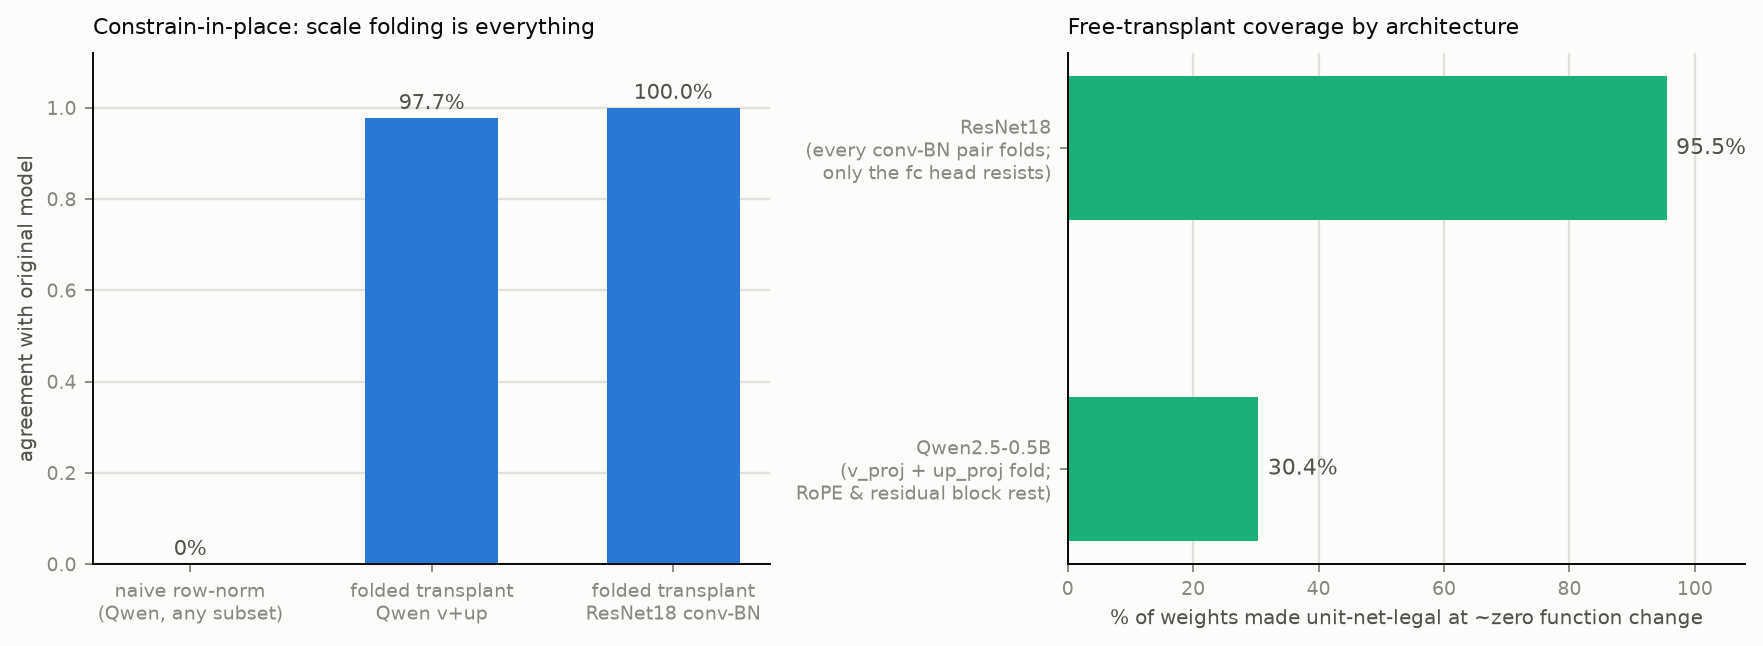
\includegraphics[width=\textwidth]{fig_transplant.png}
\caption{Constrain-in-place: folding is everything; coverage by
architecture.}
\end{figure}

\section{Idea 2 --- native integer quantization}
A convex $P$ row stored as integer numerators summing to exactly $2^b$
(largest remainder) is exact fixed-point arithmetic with a shared
denominator; $N$ takes the $2^b$ grid on $[0,1]$.

\begin{center}\small\begin{tabular}{@{}lccc@{}}\toprule
bits & LM agree & LM pos-slot & ResNet top-1\\\midrule
float32 & 0.300 & 1.00 & 0.653\\
12 & 0.302 & 1.00 & 0.653\\
10 & \textbf{0.300 (lossless)} & 1.00 & 0.410\\
8 & 0.214 & 1.00 & 0.000\\
4 & 0.096 & 1.00 & 0.000\\
2 & 0.001 & 1.00 & 0.000\\
\bottomrule\end{tabular}\end{center}

For the LM student, 10 bits is lossless \emph{and} 5$\times$ sparsifying
(3.4M $\to$ 710k nonzeros): the integer budget forces zeros, so the bit
budget \emph{is} a sparsity budget. The same coupling is a liability for
lean deep nets: ResNet's 4{,}608-weight filters amputate to $\le$256
nonzeros at 8 bits and 20 layers compound the noise. \textbf{Law: simplex
quantization needs denominator $\ge$ row length; tolerance to
constraint-native compression measures the redundancy training left
behind.}

\section{Idea 3 --- activation-flow pruning}
Importance $=$ corpus-summed activation flow per edge
($\mathbb{E}[|w|\cdot a]$); raise the floor, watch divergence. Pruned
models stay legal (P rows renormalized; for the ResNet the fresh scale
re-folds into BN, so only the pruning itself changes the function).

\begin{center}\small\begin{tabular}{@{}lcccc@{}}\toprule
edges pruned & LM agree & LM KL & LM pos-slot & ResNet top-1\\\midrule
50\% & 0.239 & 0.81 & 1.00 & 0.524\\
80\% & 0.094 & 3.77 & 1.00 & 0.103\\
90\% & 0.024 & 7.69 & 1.00 & 0.000\\
99\% & 0.000 & 15.3 & 1.00 & ---\\
\bottomrule\end{tabular}\end{center}

\begin{figure}[h]\centering
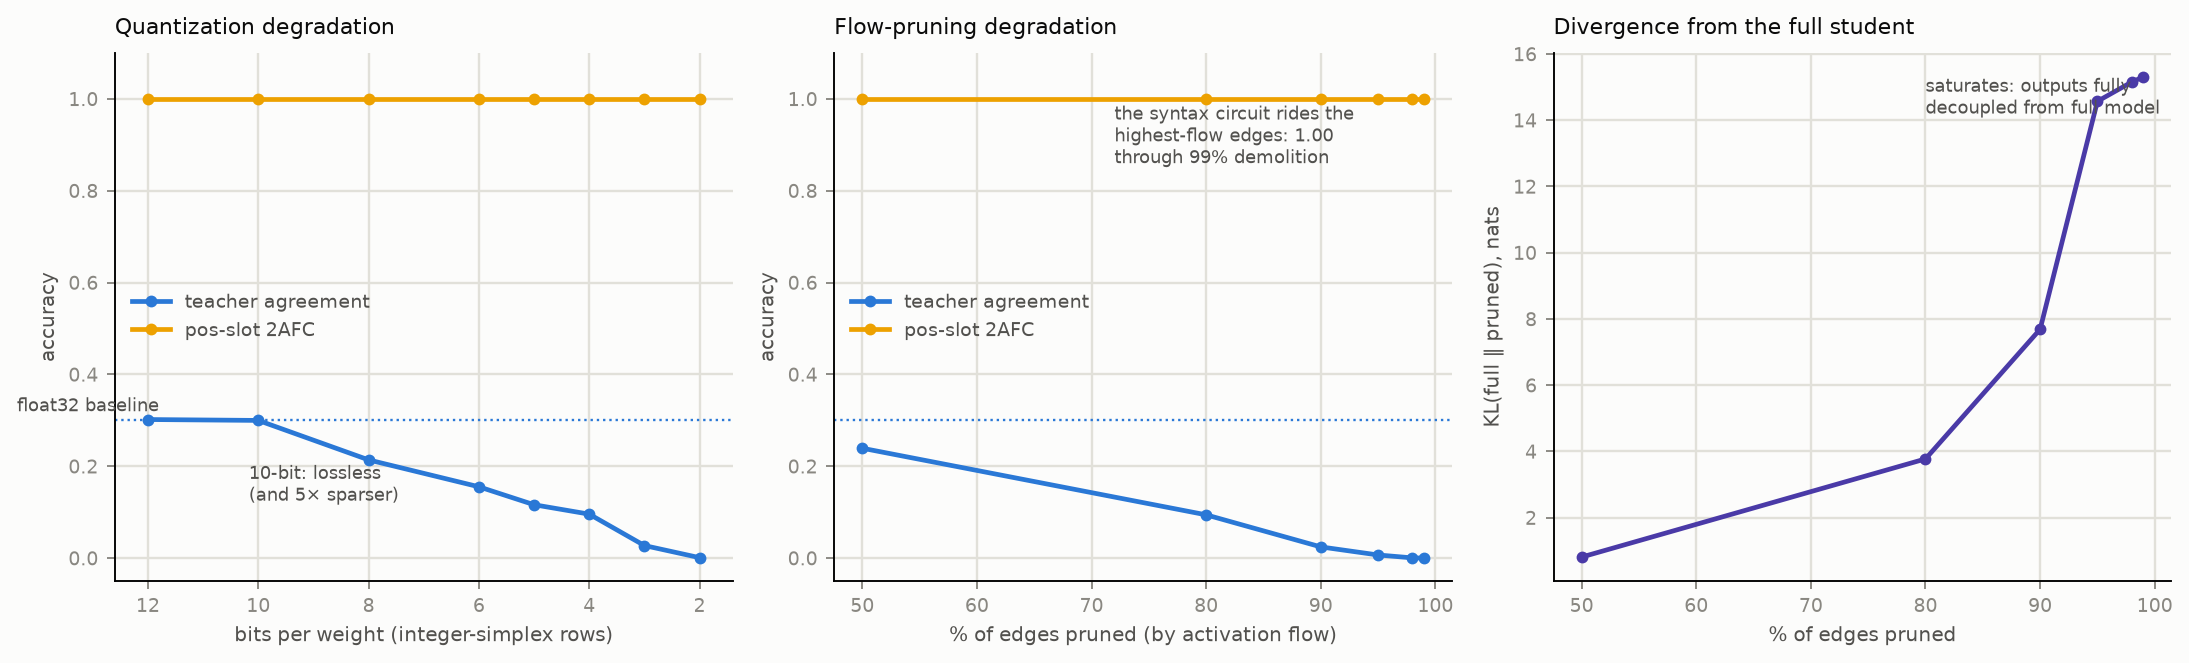
\includegraphics[width=\textwidth]{fig_degradation.png}
\caption{LM student: quantization and flow-pruning degradation;
divergence from the full model. The yellow line is \S4.}
\end{figure}
\begin{figure}[h]\centering
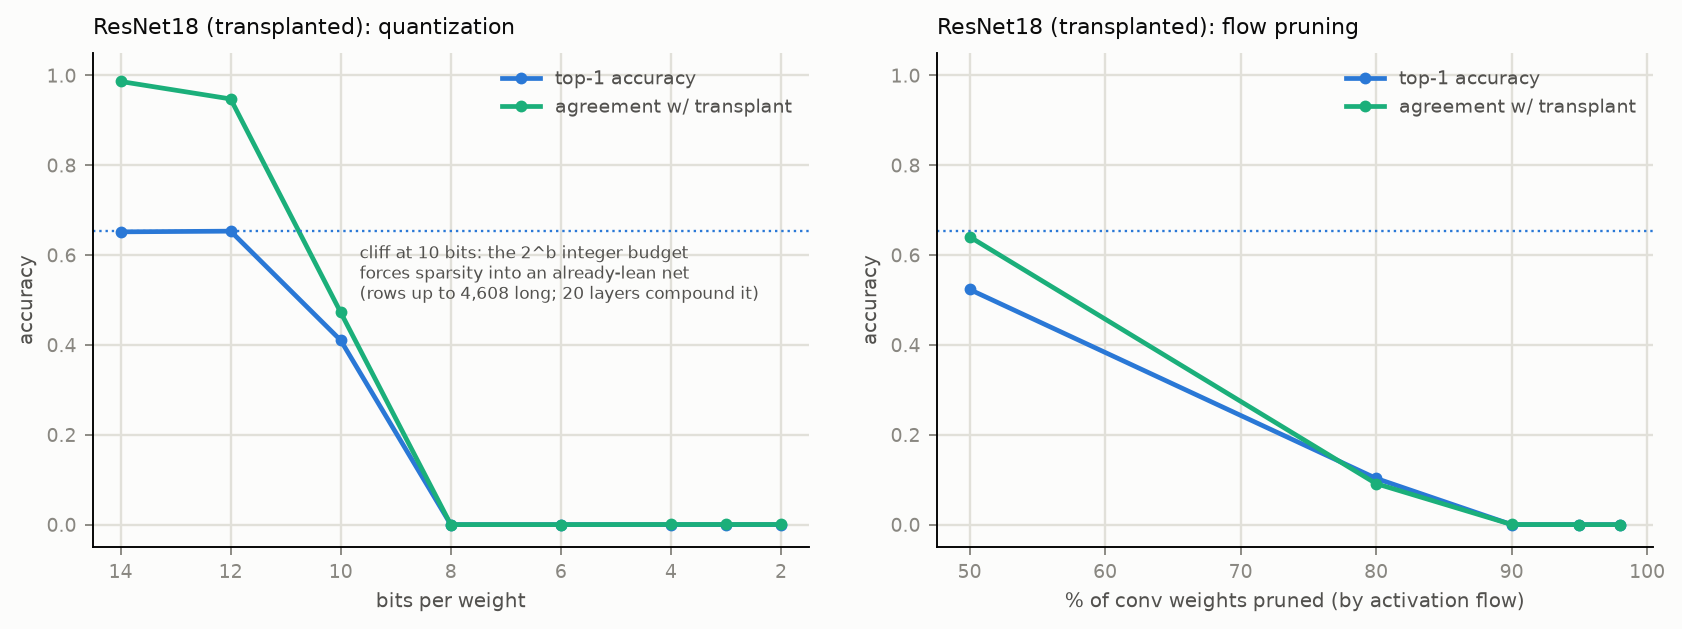
\includegraphics[width=.85\textwidth]{fig_resnet_degrade.png}
\caption{ResNet18: the same treatments; steeper everywhere --- depth
compounds and lean filters amputate.}
\end{figure}

\section{The cross-cutting finding: syntax rides the highways}
Across every destructive condition on the LM --- 2-bit quantization, 99\%
pruning, agreement statistically zero --- the pos-slot syntax task held
\textbf{1.00}. The verb/noun circuit lives on the highest-flow edges,
which every mass-respecting destruction spares last; semantic capillaries
die first. With Day 2's j-carve: targeted carving keeps the circuit at
4\% of the network \emph{on purpose}; flow-pruning keeps it at 1\%
\emph{by accident}. \emph{Syntax rides the trunk roads; meaning lives in
the side streets.}

\section{Artifacts}
Channel-level 3D explorer (3{,}917 channel-nodes, 9{,}620 edges, residual
arcs; conv1 nodes open their actual RGB $7{\times}7$ filters --- each now
a unit budget, so intensities compare across the layer):
\href{https://claude.ai/code/artifact/c51a40dc-016a-44ae-89ed-141fbd26e98a}
{artifact c51a40dc}. Voxel-level whole-net explorer (19 stages, 1{,}098
voxels lit by real activations on a church image, 13{,}784 exact
receptive-field cones as low-clearance curves, orbit+pan+zoom; weight
sharing directly visible):
\href{https://claude.ai/code/artifact/ff2ee392-5a45-4fcd-9487-f22841c0decf}
{artifact ff2ee392}. (v1's lofted arcs cached for posterity.)

\section{Standing conclusions}
(1) Constraint migration is mostly free where normalization absorbs
scale: $\sim$100\% of CNN convs, $\sim$30\% of transformer linears,
exactly, with zero clipping observed. (2) The geometry quantizes and
sparsifies as one operation, with a sharp validity condition. (3)
Robustness to native compression is a redundancy meter. (4) Functional
anatomy is stratified by flow: syntax on highways, semantics on
capillaries --- measured, not metaphor.

\textbf{Next:} constrained-finetune the transplants to retire the scale
debt; rerun the J-lens/workspace program on the transplanted ResNet
(95.5\% legal $=$ the exact lens now applies to a real ImageNet model);
j-carve Tier-1 against a transplant-initialized student.

\end{document}
